\documentclass{article}[a4paper, 12pt, italian]
\usepackage[T1]{fontenc}
\usepackage[utf8]{inputenc}
\usepackage{amsmath, amssymb, amsthm, thmtools, amsfonts, mathtools}
\usepackage{nicefrac}
\usepackage{calc}
\usepackage[pdftex, hyperindex, plainpages=false]{hyperref}
\usepackage[nameinlink]{cleveref} %load before classicthesis (clash)
%\usepackage[nochapters,pdfspacing]{classicthesis}
\usepackage{siunitx}
\usepackage[siunitx]{circuitikz}

\usepackage[a4paper]{geometry}
\usepackage{float}
\usepackage{mdframed}
\usepackage{titling}
\usepackage{booktabs}
\usepackage{graphicx}
\usepackage{caption, subcaption}
\usepackage{xcolor}
\usepackage[italian]{babel}
\usepackage{pgfplots}
\usepackage{listings}
%\usepackage{lmodern}
\usepackage{url}
\usepackage{enumitem}
\usepackage{tikz} %loads after classicthesis (xcolor incompat)

% lets graphicx know path where figures to be included are found
\graphicspath{{../figs/}}
\makeatletter
\def\input@path{{../figs/}}
%or: \def\input@path{{/path/to/folder/}{/path/to/other/folder/}}
\makeatother

% tikz pgf plots setup
\usepgfplotslibrary{external}
\pgfplotsset{compat=1.15}
%\tikzexternalize

% spaces and significant digits/figures for measurements
\sisetup{free-standing-units, space-before-unit, number-unit-product = \;,
scientific-notation = false, round-mode = figures, round-precision = 1,}

% turns all (hyperlinked) references black [default is blue]
\hypersetup{
	linktoc=all,
	colorlinks=true,
	linkcolor=black
}

% code listings config
%\lstset{
%language=Python,
%basicstyle=\ttfamily,
%columns=fullflexible,
%keepspaces=true,
%}

% mdframed (for boxed text) configuration
\mdfsetup{linewidth=0.6pt}

% Default fixed font does not support bold face
\DeclareFixedFont{\ttb}{T1}{txtt}{bx}{n}{12} % for bold
\DeclareFixedFont{\ttm}{T1}{txtt}{m}{n}{12}  % for normal

% Custom colors
\usepackage{color}
\definecolor{deepblue}{rgb}{0,0,0.5}
\definecolor{deepred}{rgb}{0.6,0,0}
\definecolor{deepgreen}{rgb}{0,0.5,0}

% Commands 
\newcommand{\executeiffilenewer}[3]{%
	\ifnum\pdfstrcmp{\pdffilemoddate{#1}}%
		{\pdffilemoddate{#2}}>0%
	{\immediate\write18{#3}}\fi%
}
% input .svg --> .pdf_tex graphs
%\newcommand{\includesvg}[1]{%
%	\executeiffilenewer{#1.svg}{#1.pdf}%
%	{inkscape -z -D --file=#1.svg %
%	--export-pdf=#1.pdf --export-latex}%
%	\input{#1.pdf_tex}%
%}
% Thanks UniPi's Department of Physics E. Fermi
\newcommand{\thanksdf}{(\thanks{Dipartimento di Fisica E.~Fermi,%
Universit\`a di Pisa - Pisa, Italy.}\;)}

% hyperlink to email address
\newcommand{\mail}[1]{\href{mailto:#1}{\textsf{#1}}}

% \vec for bold vectors, instead of overarrows (now "\arrvec")
\let\arrvec=\vec
\renewcommand{\vec}[1]{\boldsymbol #1}
% replaces straight phi with slanted phi
\renewcommand{\phi}{\varphi}
% replaces straight eps with curved epsilon
\newcommand{\eps}{\varepsilon}
% abbreviation for (sub_/super^)scripts of \lim, \sum,... in inline math
\newcommand{\ds}{\displaystyle}

% blackboard/number set letters
\newcommand{\CC}{\mathbb C}
\newcommand{\HH}{\mathbb H}
\newcommand{\KK}{\mathbb K}
\newcommand{\NN}{\mathbb N}
\newcommand{\PP}{\mathbb P}
\newcommand{\QQ}{\mathbb Q}
\newcommand{\RR}{\mathbb R}
\newcommand{\ZZ}{\mathbb Z}

\newcommand{\Abs}[1]{{\left\Vert #1\right\Vert}}
\newcommand{\enclose}[1]{{\left( #1 \right)}}
\newcommand{\Enclose}[1]{{\left[ #1 \right]}}
\newcommand{\floor}[1]{\left\lfloor #1 \right\rfloor}
\newcommand{\ceil}[1]{\left\lceil #1 \right\rceil}
\newcommand{\To}{\rightrightarrows}

% Math operators
\DeclareMathOperator{\divergence}{div}
\renewcommand{\div}{\divergence}
\DeclareMathOperator{\Imaginarypart}{Im}
\renewcommand{\Im}{\Imaginarypart}
\DeclareMathOperator{\Realpart}{Re}
\renewcommand{\Re}{\Realpart}
%\DeclareMathOperator{\arg}{arg}
\DeclareMathOperator{\tg}{tg}
\DeclareMathOperator{\arctg}{arctg}
\DeclareMathOperator{\settsinh}{settsinh}
\DeclareMathOperator{\settcosh}{settcosh}
\DeclareMathOperator{\tr}{tr}
\DeclareMathOperator{\im}{im}
\DeclareMathOperator{\sgn}{sgn}
\DeclareMathOperator{\diag}{diag}

\DeclarePairedDelimiter{\norm}{\lVert}{\rVert}
\DeclarePairedDelimiter{\scalar}{\langle}{\rangle}

% Logarithm with arbitrary base.
% -> log_10
\newcommand{\llog}[1][10]{\log_{#1}}

% Absolute value.
% -> |x|
\newcommand{\abs}[1]{\left| #1 \right|}

% Powers.
% -> x^a
\newcommand{\power}[2][2]{\left( #2 \right)^{#1}}

% Square.
% -> x^2
\newcommand{\sq}[1]{\power[2]{#1}}

% Expansion of the binomial coefficient.
% -> n1!/(n2!(n1 - n2)!)
\newcommand{\binomexpr}[2]{\frac{#1!}{#2!(#1 - #2)!}}

% Expression evaluation at a given point with square brackets.
% -> [x]_{a}
\newcommand{\at}[2]{\left[ #1\right]_{\makebox[-1pt][l]{${\scriptstyle#2}$}}}

% Expression evaluation in an interval.
% -> [x] _{a}^{b}
\newcommand{\eval}[3]{\left.#1%
  \right|_{\makebox[-1pt][l]{${\scriptstyle#2}$}}^{\makebox[-1pt][l]{${\scriptstyle#3}$}}}

% Upright d in math mode (for differentials).
% -> d
\newcommand{\ud}{\mathrm{d}}

% Differential.
% -> dx
\newcommand{\diff}[1][x]{\,\ud{#1}}

% Base command for defining derivatives.
% -> df/dx or d^kf/dx^k
\newcommand{\basederivative}[4][]{%
  \displaystyle%
  \ifx\\#1\\\frac{#4#2}{#4#3}%
  \else%
  \frac{#4^#1#2}{#4#3^#1}%
  \fi%
}

% Total derivative.
% -> df/dx(x) or d^kf/dx^k(x)
\newcommand{\td}[4][]{%
  \basederivative[#1]{#2}{#3}{\ud}%
  \ifx\\#4\\%
  \else%
  \mkern-4mu\left(#4\right)%
  \fi%
}

% Partial derivative.
% -> df/dx(x) or d^kf/dx^k(x)
\newcommand{\pd}[4][]{%
  \basederivative[#1]{#2}{#3}{\partial}%
  \ifx\\#4\\%
  \else%
  \mkern-4mu\left(#4\right)%
  \fi%
}

\newcommand{\intinf}{\int_{-\infty}^{\infty}\!\!\!}

\newcommand{\cinterval}[2]{\left[\, #1,~#2 \,\right]}

\newcommand{\linterval}[2]{\left[\, #1,~#2 \,\right)}

\newcommand{\rinterval}[2]{\left(\, #1,~#2 \,\right]}

\newcommand{\ointerval}[2]{\left(\, #1,~#2 \,\right)}

\newcommand{\prob}[1]{\displaystyle P\left(#1\right)}

\newcommand{\pvalue}{\emph{$p$-value}}

\newcommand{\cond}{\,|\,}

\newcommand{\expect}[1]{\displaystyle E\left[#1\right]}

\newcommand{\mom}[2][]{\displaystyle {\cal M}_{#2}\ifx\\#1\\\else(#1)\fi}

\newcommand{\momalg}[1]{\displaystyle \lambda_{#1}}

\newcommand{\momcen}[1]{\displaystyle \mu_{#1}}

\newcommand{\skewness}{\displaystyle \gamma_1}

\newcommand{\kurtosis}{\displaystyle \gamma_2}

\newcommand{\charf}[1][x]{\phi_{#1}}

\newcommand{\momgenf}[1][x]{M_{#1}}

\newcommand{\fwhm}{{\scriptstyle \textsc{FWHM}}}

\newcommand{\hwhm}{{\scriptstyle \textsc{HWHM}}}

\newcommand{\median}{\mu_{\nicefrac{1}{2}}}

\newcommand{\var}[1]{\ensuremath{\text{Var}\left(#1\right)}}

\newcommand{\cov}[2]{\ensuremath{\text{Cov}\left(#1, #2\right)}}

\newcommand{\corr}[2]{\ensuremath{\text{Corr}\left(#1, #2\right)}}

\newcommand{\like}{\mathcal L}

\newcommand{\likelihood}[2][]{\like\ifx\\#2\\\else(#2\ifx\\#1\\\else;#1\fi)\fi}

\newcommand{\chisq}{\ensuremath{\chi^2}}

\newcommand{\chisquare}[2][]{\chisq\ifx\\#2\\\else(#2\ifx\\#1\\\else;#1\fi)\fi}

\newcommand{\loglikelihood}[2][]{\log\likelihood[#1]{#2}}

\newcommand{\pdf}[3][]{#2(#3\ifx\\#1\\\else;#1\fi)}

\newcommand{\binomialpdf}[2][]{\pdf[#1]{\mathcal B}{#2}}

\newcommand{\multinomialpdf}[2][]{\pdf[#1]{\mathcal M}{#2}}

\newcommand{\poissonpdf}[2][]{\pdf[#1]{\mathcal P}{#2}}

\newcommand{\uniformpdf}[2][]{\pdf[#1]{u}{#2}}

\newcommand{\exponentialpdf}[2][]{\pdf[#1]{\varepsilon}{#2}}

\newcommand{\gausspdf}[2][]{\pdf[#1]{N}{#2}}

\newcommand{\chisquarepdf}[2][]{\pdf[#1]{\wp}{#2}}

\newcommand{\cauchypdf}[2][]{\pdf[#1]{c}{#2}}

\newcommand{\erf}[1]{\ensuremath{\text{erf}\left(#1\right)}}

\newcommand{\dccases}[4][]{#2 \ifx\\#2\\\else=\fi %
  \begin{cases}
    \displaystyle #3 & \text{per variabili discrete}\\
    \displaystyle #4 & \text{per variabili continue}#1
  \end{cases}
}
% sub/super-scriptable for all symbol as math operator 
\newcommand\Scaleforall[1]{\vcenter{\hbox{\scalefont{#1}$\forall$}}}

\DeclareMathOperator*\forevery{%
  \vphantom\sum
  \mathchoice{\Scaleforall{2}}{\Scaleforall{1.4}}{\Scaleforall{1}}{\Scaleforall{0.75}}}

% adjustable page margins, currently scientific article standards
\geometry{left=25mm, right=25mm, top=25mm, bottom=25mm}

\title{Esercitazione 0 di Laboratorio 3}
\author{B.~Tomelleri\thanksdf \and M.~Rossi(\protect\footnotemark[1] )}
\date{\today}

\begin{document}
\maketitle

%================================================================
%                         Introduzione
%================================================================
\section{Introduzione}
Scopo dell’esercitazione è di acquisire familiarità con le funzionalità
di Waveforms come oscilloscopio e generatore di funzioni.

%================================================================
%                         Cenni teorici
%================================================================
\section{Cenni Teorici}

%================================================================
%                Metodo e apparato sperimentale
%================================================================
\section{Metodo e apparato sperimentale}
Digilent AD2 e applicazione dedicata Waveforms

%================================================================
%                   Analisi dati e Risultati
%================================================================
\section{Analisi dati e Risultati}

Da un \emph{fit} con un modello:
\begin{lstlisting}
def dosc(t, A, frq, phi, ofs, tau):
    return A*np.exp(-t/tau)*np.cos(2*np.pi*frq*t + phi) + B
\end{lstlisting}

Lasciando liberi tutti i parametri $A$, $\omega$, $\tau$ $\phi$ e $B$
(e propagando gli errori sulla variabile indipendente) si ottengono i valori:
\begin{align*}
A &= 1.2045 \pm 0.0007  \; \si{\volt} \qquad &B &= -73.27 \pm 0.02 \;
\si{m\volt} \\
f &= 5722 \pm 1 \; \si{\hertz} \qquad &\phi &= 311 \pm 2 \; \si{m\radian} \\  
\tau &= 88.41 \pm 0.02 \; \si{\us} \qquad &Q_f &= 1.6 \pm 0.2 \\
\rm{norm\_cov_{(A, f)}} &= 0.71 \qquad &\rm{norm\_cov_{(A, B)}} &= -0.03 \\
\rm{norm\_cov_{(A, \tau)}} &= -0.73 \qquad &\rm{norm\_cov_{(A, \phi)}} &= -0.85 \\ 
\rm{norm\_cov_{(f, \phi)}} &= -0.84 \qquad &\rm{norm\_cov_{(f, \tau)}} &= -0.59 \\
\rm{norm\_cov_{(f, B)}} &= -0.02 \qquad &\rm{norm\_cov_{(\phi, B)}} &= 0.02 \\
\rm{norm\_cov_{(\phi, \tau)}} &= 0.53 \qquad &\rm{norm\_cov_{(B, \tau)}} &= 0.05 \\
\chi^2 &= 215.4/245 \qquad &\rm{abs\_sigma} &= \rm False
\end{align*}

Ed il grafico \ref{plt:rlcfit}\\
\begin{figure}[!htb]
	\centering 
 		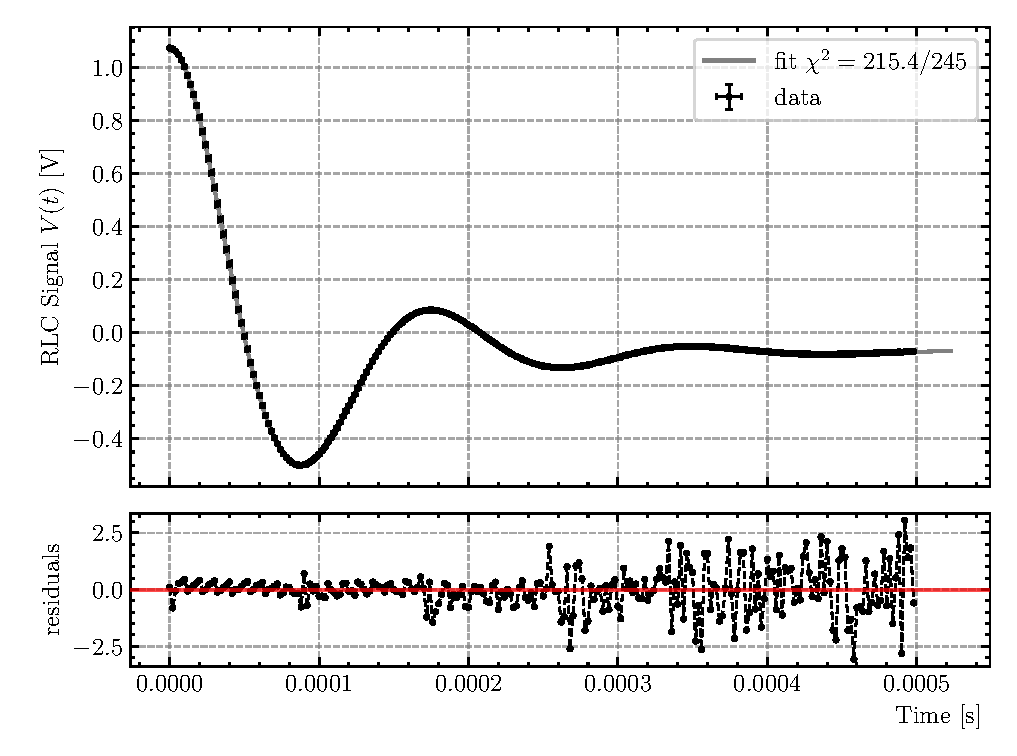
\includegraphics[scale=0.9]{rlcfit}
    \caption{Fit del segnale $V(t)$ rispetto al tempo \label{plt:rlcfit}}
\end{figure}
% Alternatively
%\begin{figure}[!htb]
%	\centering 
% 		\includegraphics[scale=0.9]{./figs/dist.pdf}
% 	\caption{Distribuzione delle • per $• = • \pm • \rm •$ \label{dist:1}}
%\end{figure}
In entrambi casi impostando $\rm{abs\_sigma} = \rm False$ in quanto l'errore
non statistico è predominante sulle misure.

% Alternatively
%\lstinputlisting[language=Python, firstline=38, lastline=39]{../foo.py}
%or even
%\begin{align*}
%\rm def\; &foo(•_{•}, •_{•}, •_{•}):\\
%    &\rm return\; •_{•}/•_{•} + •_{•}
%\end{align*}

\subsection{Nota sul metodo di fit}
Per determinare i parametri ottimali e le rispettive covarianze si \`e
implementato in \verb+Python+ un algoritmo di fit basato sui minimi quadrati
mediante la funzione \emph{curve\_fit} della libreria 
\texttt{SciPy}\cite{scipy}.
%================================================================
%                          Conclusioni
%================================================================
\section{Conclusioni}
La forma d'onda oscillante ha si spegne dopo qualche periodo, per cui
il fattore di merito trovato è ragionevole, essendo maggiore del valore
$Q_c = \nicefrac{1}{2}$ corrispondente a smorzamento critico del sistema,
ma comunque dello stesso ordine di grandezza.
\bibliography{../../latex/refs}
\end{document}
